\documentclass[a4paper,12pt]{article}

% Pakete
\usepackage[utf8]{inputenc}
\usepackage[english]{babel} % Deutsche Sprache
\usepackage{graphicx} % Für Bilder
\usepackage{amsmath} % Für mathematische Formeln
\usepackage{booktabs} % Für Tabellen
\usepackage[hidelinks]{hyperref} % Für Hyperlinks
\usepackage{listings} % Für Code-Blöcke
\usepackage{minted} % Auch für Code-Blöcke
\usepackage{caption}
\usepackage{menukeys}
\usepackage{float}
\usepackage{enumitem}
\usepackage{tocloft}
\usepackage{pgfplots}
\usepackage{pgfplotstable}
\usepgfplotslibrary{groupplots}
\usepackage{siunitx}
\usepackage{multicol}
\usepackage{xcolor}
\usepackage{tikz}
\usepackage{textcomp}
\newcommand{\mytexttilde}{\raisebox{0.5ex}{\texttildelow}}

\usepackage{fancyhdr}
\pagestyle{fancy}

\fancyhf{} % löscht alle aktuellen Kopf- und Fußzeilen

% Kopfzeile: linke Seite = aktuelle Section
\fancyhead[L]{\nouppercase{\leftmark}}

% Fußzeile: linke Seite = Name, rechte Seite = FH Salzburg, zentriert = Seitenzahl
\fancyfoot[L]{Marc Toiflhart, Sebastian Maier}
\fancyfoot[C]{\thepage}
\fancyfoot[R]{Högskolan i Halmstad}

\usepackage{placeins}

\usepackage[
backend=biber,
style=ieee,
sorting=ynt
]{biblatex}

\renewcommand{\listingscaption}{Sourcecode}

\addbibresource{literatur.bib}

\begin{document}

\begin{titlepage}
    \centering
    
\includegraphics[width=5cm]{Resources/hogskolan-halmstad-logo.png} \\[0.5cm] % Logo
    Högskolan i Halmstad \\[0.2cm]
    Biometric Recognition \\[1.5cm]
    
    \hrule
    \vspace{0.4cm} % statt \\[0.4cm]
    {\LARGE \textbf{Laboratory Report}}
    \vspace{0.4cm}
    \hrule
    \vspace{1.5cm} % statt \\[1.5cm]

    {\Large \textbf{Biometric Recognition Laboratory}} \\[0.2cm]
    {\Large Hand Geometry} \\[1cm]
    
    \textbf{Author:} Marc Toiflhart, Sebastian Maier \\[0.2cm]
    \textbf{Date:} \today \\[0.2cm]
    \textbf{Supervisor:} Kevin Hernández Diaz

    \vfill
\end{titlepage}
\newpage

\begin{center}
    \textbf{Summary}
\end{center}
In diesem Labor wurden Videosequenzen mit dem H.264-Codec unter variierenden Bitraten, Quantisierungsparametern und Presets kodiert und hinsichtlich Qualität und Kodierzeit analysiert. Ergänzend wurde ein C-Programm zur Einlesung und Verifikation von IYUV-Daten sowie zur Motion Estimation mit verschiedenen Metriken entwickelt.

\vspace{0.4cm} % statt \\[0.4cm]
\centering
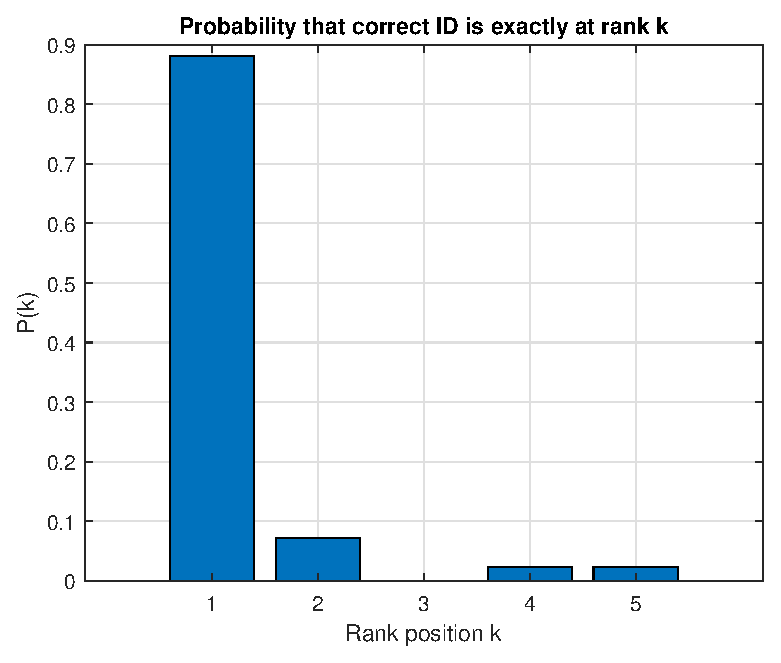
\includegraphics[width=5cm]{Resources/rank_plot.eps} \\[0.5cm]

\newpage
\section{Measure hand properties}
%Aufgabenstellung:
Measure in each image provided, the hand geometry properties (finger’s length and width, palm width, etc.) according to the "measuring template" attached with the exercise. Use a ruler and measure in mm, e.g. 20 mm. You will then obtain four feature vectors E1, E2, E3 and E4, one for each image.


\section{Identification exercise}

\subsection{Calculating P(k) by hand}
%Aufgabenstellung:
Calculate by hand the function P (k) for k = 1, 2, ....P (k) indicates the chance (probability) that the correct identity is output in position k of IdLista. Draw the function P(k) that you calculated in a graph.

\subsection{Calculating TPIR (M) and plotting CMC curve}
%Aufgabenstellung:
Calculate by hand the function TPIR (M) and draw it in a graph (the CMC curve). 
TPIR (M) indicates the chance (probability) that the correct identity is output in the first M positions of the output list.  TPIR (M) is obtained by summing up P(k) up to k = M.
Put also the values of P (k) and TPIR (M) in a table.


\subsection{List Length for 90\% Identification Probability}
%Aufgabenstellung:
From TPIR (M), calculate the length of the list M to have a 90\% chance that the correct identity is obtained in IdLista among the first M identities.

\subsection{Most and Least Similar IDs with Distances}
%Aufgabenstellung:
Find the two ID numbers that are the most and the least similar to your own ID. Also write down the distances of the two cases (how similar the hands are).


\section{Verification exercise}

\subsection{FAR and FRR Calculation from Genuine and Impostor Distances}
%Aufgabenstellung:
With the help of the histograms you created earlier and shown in Figure = 100 (Genuine class) and figure = 101 (Impostor class), calculate and plot the probability of the FA error (= FAR) and FR error (= FRR) for various thresholds. You can also work directly with the distances in the vectors ShDist (Genuine) and OhDist (Impostor). Create a table with different thresholds and the number of errors of each type.

\subsection{FR Error Calculation and Threshold Variation}
%Aufgabenstellung:
A Matlab command that you can use to calculate the number of FR errors at a specific threshold Th is: sum (ShDist> Th). Vary the value of Th and annotate both Th and the number of FR errors in a table.


\subsection{FRR Computation and Plotting vs. Threshold}
%Aufgabenstellung:
How can you compute the probability (Slh) from the number of FR errors, i.e. FRR? Calculate FRR for each value of Th and annotate the FRR in the table. Now you can plot the FRR for different values of the threshold Th! Use Matlab function plot for this purpose.

\subsection{FAR Calculation for Impostor Class}
%Aufgabenstellung:
Create a similar table and graph of the class Impostor. Which is the Matlab command to compute FA errors using OhDist and Th?


\subsection{FRR and FAR Tables and Figure}
%Aufgabenstellung:
Present the estimated errors (FRR and FAR for different values of Th) of the system in two tables and in a figure as Figure 6.

\subsection{EER Estimation and Threshold Selection}
%Aufgabenstellung:
From your results, indicate the approximate value of the EER (Equal Error Rate). Suggest also suitable values of Th for: 1) high security requirement, and 2) high convenience requirement. Indicate the value of Th, FAR and FRR for every case 1) and 2).



% Inhaltsverzeichnis
\tableofcontents
\newpage

% Abbildungsverzeichnis
\listoffigures
\newpage

% Tabellenverzeichnis
\listoftables
\newpage


\newpage
\printbibliography

\end{document}